\subsection{Processadores}
A \emph{CPU} (\emph{Central Process Unit} -  no portugues Unidade Central de Processamento) muitas vezes é considerado o cérebro do computador ela é responsável por receber as instruções da memória e processá las, decodificando-as e executando todos os processos em fila de execução num ciclo que é repetido até que o programa termine \cite{Tanenbaum2016}. \\
Assim os programas são executados. Cada \emph{CPU} é presa a sua arquitetura assim não conseguindo decodificar instruções de arquiteturas diferentes como \emph{ARM} para X86 ou vice e versa. A velocidade de cálculo das \emph{CPU`s} é muito maior que o tempo para executar uma instrução registradores internos são utilizados para armazenamento de variáveis e resultados temporários \cite{Tanenbaum2016}.\\
O SO deve conhecer absolutamente todos os processos destinados ao processador e também todos os registradores gerados pois quando a \emph{CPU} realiza uma multiplexação ela interrompe o programa em execução para recomeçar outro. Assim faz-se necessário que o SO tem que salvar todos os registradores de maneira que eles possam ser restaurados quando o programa for executado mais tarde. Muitas \emph{CPU`s} modernas têm recursos para executar mais de uma instrução ao mesmo tempo \cite{Tanenbaum2016}. \\
Por exemplo, uma \emph{CPU} pode ter unidades de busca, decodificação e execução separadas, assim enquanto ela está executando a instrução não, poderia também estar decodificando a instrução n + 1 e buscando a instrução n + 2. Uma organização com essas características é chamada de \emph{pipeline} como na figura \ref{fig:Processador1} abaixo \cite{Tanenbaum2016}.\\
\begin{figure}[htpb]
    \centering
   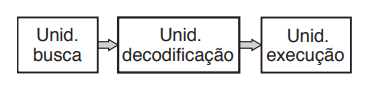
\includegraphics[scale=1]{imagens/Processador1.png}
   \caption{Um \emph{pipeline} com três estágios. \cite{Tanenbaum2016}}
   \label{fig:Processador1}
\end{figure}\\

Ainda mais avançada que um projeto de \emph{\emph{pipeline}} é uma \emph{CPU} superescalar, mostrada na Figura \ref{fig:Processador2}. Nesse projeto, unidades múltiplas de execução estão presentes. Uma unidade para aritmética de números inteiros, por exemplo, uma unidade para aritmética de ponto flutuante e uma para operações booleanas. Duas ou mais instruções são buscadas ao mesmo tempo, decodificadas e jogadas em um \emph{buffer} de instrução até que possam ser executadas. Tão logo uma unidade de execução fica disponível, ela procura no buffer de instrução para ver se há uma instrução que ela pode executar e, se assim for, ela remove a instrução do \emph{buffer} e a executa \cite{Tanenbaum2016}. 
\begin{figure}[htpb]
    \centering
   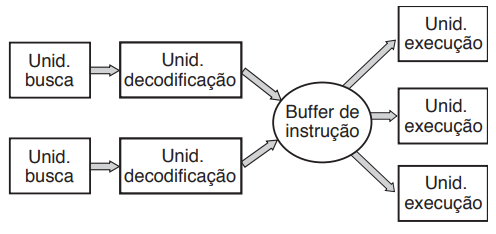
\includegraphics[scale=1]{imagens/Processador2.png}
   \caption{Uma \emph{CPU} superescalar. \cite{Tanenbaum2016}}
   \label{fig:Processador2}
\end{figure}\\

Um \emph{thread} é um tipo de processo leve, mais para o SO cada \emph{thread} é como uma \emph{CPU} separada, considere um sistema com duas \emph{CPU`s} efetivas, cada uma com dois threads. O sistema operacional verá isso como quatro \emph{CPU`s} chamamos isso de \emph{multithreading} \cite{Tanenbaum2016}.